Como apresentado na Se��o (\ref{section:Cordic}), devido a limita��es em disponibilidade de blocos multiplicadores nas FPGAs, se faz necess�rio ultilizar o algoritmo Cordic implementado em \textit{hardware} para realizar as opera��es de rotacionamento do vetor $H_r$ pelo �ngulo descrito por $W_{N_o}^r$. 

A FPGA XC7Z010-1CLG225 possui ao total 80 blocos de DSP (\textit{Digital signal processing}), onde cada um deles possui um \textit{hardware} multiplicador. Tais multiplicadores seriam suficientes para implementar a fun��o de rota��o de vetores necess�ria ao c�lculo da FFT. Por�m como tais blocos est�o em pequena quantidade e s�o essenciais para uma vasta gama de aplica��es. Como a FFT � um recurso que raramente � implementado isoladamente, sendo mais comum encontrar a FFT como apenas um dos elementos constituintes de um aplica��o bem maior, evitar o uso de DSP para reserva-los a outros sistemas � pertinente.    

Nesta etapa ser� realizado o projeto e implementa��o em FPGA do processador Cordic utilizado para montar o bloco da FFT. Tal processador seguira o funcionamento do algoritmo MSR Cordic apresentado na Se��o (\ref{section:MSR-CORDIC}).

\section{Projeto dos Par�metros Cordic}

Como apresentado na Se��o (\ref{section:MSR-CORDIC}), a determina��o dos par�metros Cordic $\mu_i$, $\mu_j$, $s_i$, $s_j$, $I$ e $J$ da Equa��o (\ref{eq:MSR}) � feita com base na minimiza��o do erro de aproxima��o $\upepsilon$, descrito pela Equa��o (\ref{eq:OtimizacaoMSR}).
Para encontrar o conjunto �timo de par�metros Cordic � poss�vel utilizar uma variedade de algoritmos determin�sticos, j� que este sistema se assemelha a problemas cl�ssicos de otimiza��o. 

Na Se��o (\ref{section:TBS}) fora apresentado o algoritmo de otimiza��o TBS, o qual se destinava a determina��o do conjunto de par�metros Cordic para o EEASR. O EEASR possu� um conjunto de �ngulos elementares menores do que o MSR, e a fun��o de otimiza��o n�o inclu�a a redu��o do do erro de ganho $K_c$ em rela��o a unidade, j� que a compensa��o deste ganho era realizada em uma etapa independente atrav�s de uma pseudo-rota��o. Por�m ao se adaptar a equa��o de minimiza��o do TBS para o caso do MSR, e incluir no conjunto de solu��o os �ngulos elementares do MSR.

Segue abaixo o pseudo-c�digo utilizado para obter o conjunto �timo de par�metros Cordic. O vetor $r_{\theta}$ representa o conjunto de todos �ngulos elementares, e $r_p$ presenta o conjuntos dos ganhos $K_n$, ambos oriundos das diferentes combina��es entre os par�metros Cordic.

 
\vspace{3mm}
	\lstset{style=VHDL}
	\begin{lstlisting}[mathescape]
		% Inicializa��o
		$\displaystyle \phi_{\theta}(1,k)~=~r_{\theta}(k)~para~todo~k,$
		$\displaystyle \phi_p(1,k)~=~r_p(k)~para~todo~k,$
		
		%Acumula��o
		$\displaystyle FOR~i=1~to~N-1$
			$\displaystyle FOR~k=1~to~Z(S_2)$
				$\displaystyle Encontra~k'~tal~que~:$
					$\displaystyle \upepsilon ~=~ min \sqrt{(\phi_{\theta}(i,k')+r_{\theta}(k)-\theta )^2 + (\phi_p(i,k^*)*r_p(k)-1 )^2} : 1 \leq k^* \leq Z(S_3) $
				$\phi_{\theta}(i+1,k)~=~\phi_{\theta}(i,k')+r_{\theta}(k)$
				$\phi_p(i+1,k^*)~=~\phi_p(i,k^*) * r_p(k)$
			$\displaystyle END$
		$\displaystyle END$
		
		%Determina��o do �timo Global
		$\displaystyle Encontra~k^*~tal~que~$
			$\displaystyle \upepsilon ~=~ min \sqrt{(\phi_{\theta}(N,k^*)-\theta )^2 + (\phi_p(N,k^*)-1 )^2} : 1 \leq k^* \leq Z(S_3) $
		$\displaystyle Result(N)~=~K^*$
		
		%Determina��o do Caminho Solu��o
		$\displaystyle FOR~i=N~to~2$
			$\displaystyle Encontra~k'~tal~que~$
				$\displaystyle \upepsilon ~=~ min \sqrt{(\phi_{\theta}(i-1,k')+r_{\theta}(k)-\theta )^2 + (\phi_p(i-1,k^*)*r_p(k)-1 )^2} : 1 \leq k^* \leq Z(S_3) $
			$\displaystyle k^*=k'$
			$\displaystyle Result(i-1)=k'$
		$\displaystyle END$
	
	\end{lstlisting}
	\label{code:PCTBSAlterado}
\vspace{3mm}

Uma aten��o especial � dada para o vetor de �ngulos elementares $r_{\theta}$. Este vetor � preenchido com o valor de �ngulos obtidos pelo conjunto de combina��es poss�veis dos par�metros Cordic do MSR, atrav�s da Equa��o (\ref{eq:S3}), o qual � reescrita como:

\begin{eqnarray}
	\alpha = \sum_{i=1}^{I} \mu_{i}2^{-s_i (n)} \\
	\beta = \sum_{j=1}^{J} \mu_{j}2^{-s_j (n)} \\
	r_{\theta} =  tan^{-1} \left(\frac{\beta}{\alpha}\right) \\ 
	:~\mu_{i},\mu_{j} \in \{-1,0,1\} \\
	s_i,s_j \in \{0,1, \dots, S\} 
	\label{eq:S32}
\end{eqnarray}

Atrav�s das diferentes combina��es de par�metros uma variedade de possibilidades de �ngulos preenchem o vetor  $r_{\theta}$. Por�m h� um problema com o c�lculo do arco tangente para combina��es onde o  $(\alpha<0, \beta<0)$ e $(\alpha>0, \beta<0)$, pois nestes casos as opera��es de rota��o deslocariam o vetor para o 4� e  3� quadrantes respectivamente, o que deveria resultar em valores de �ngulos maiores que $\pi/2$. Por�m o arco tangente considera apenas valores dentro do intervalo $(-\pi/2, \pi/2)$. Para corrigir tal efeito basta aplicar a seguinte condi��o:

\begin{eqnarray}
	Se~\alpha<0~e~\beta<0:~~r_{\theta} =  tan^{-1} \left(\frac{\alpha}{\beta}\right) -\frac{\pi}{2} \\ 
	Se~\alpha<0~e~\beta>0:~~r_{\theta} =  tan^{-1} \left(\frac{\alpha}{\beta}\right) +\frac{\pi}{2} \\ 
\end{eqnarray}  
 
Alguns par�metros do MSR s�o determinados de acordo com as limita��es de complexabilidade e disponibilidade de \textit{hardware}, como � o caso do n�mero de itera��es Cordic $N$, o n�mero de termos SPT $N_{SPT}$, e o n�mero m�ximo de deslocamentos de \textit{bit} $S$. Para alguns valores fora observado a recomenda��o usual na literatura, em \cite{Chih}, \cite{Kuo}, \cite{Park} e \cite{Kamal}. 

O n�mero de itera��o Cordic $N$ impacta diretamente no n�mero de ciclos de \textit{clock} necess�rio para realizar a opera��o, e tamb�m impacta no erro final $\upepsilon$. Como observado em \citeonline{Chih}, � admiss�vel tomar $N$ como 3, e ainda obter um bom SQNR. J� o $N_{SPT}$ impacta tamb�m no desempenho do erro $\upepsilon$, mas afeta ainda a complexabilidade do \textit{hardware}, j� que mais termos SPT significa mais operadores de deslocamento de \textit{bit}. Como a inten��o � montar uma FFT de bom desempenho, com o maior n�mero de pontos poss�vel, $N_{SPT}=3$ � admiss�vel baseado no que � visto em \citeonline{Chih}.

A escolha do n�mero m�ximo de deslocamento de \textit{bits} $S$ plica na utiliza��o de \textit{barrel shifters} maiores, e tamb�m no aumento do volume de mem�ria necess�ria para guardar os conjuntos de par�metros Cordic, para utilizar durante as opera��es de rota��o. Quanto maior for $S$ mais liberdade � dado ao conjunto de �ngulos elementares, e mais f�cil � encontrar conjuntos que reduzam $\upepsilon$ dentro das restri��es. 

A arquitetura da FFT implementada neste trabalho � pensada de modo que o fluxo de dados de entrada possam vir do Sistema de Processamento (PS), mas tamb�m possibilite a entrada de dados advinda de ADC (\textit{Analog-to-digital Conversor}) Flash de \textit{bits} bits. Portanto as palavras bin�rias utilizadas para representar os sinais precisam ter no m�nimo 12 \textit{bits}.  Para evitar a ocorr�ncia de \textit{overflow} em uma estrutura como a FFT de 1024 pontos, onde h� 10 n�veis, e apenas um ponto de soma a cada n�vel, e os ganhos s�o pr�ximos da unidade, se faz necess�rio utilizar 16 \textit{bits} para a representa��o de sinais.

Logo para determinar um valor para $S$, foi implementado o Algoritmo (\label{{code:PCTBSAlterado}}) com auxilio do \textit{software} $Matlab^\circledR$. Para cada valor de $S \in \{1...16\}$ fora criado conjunto de par�metros Cordic, fixando $I=1$ e $J=2$ (Modo Normal), para a partir destes par�metros realizar opera��es de rotacionamento de vetores nos moldes da Equa��o (\ref{eq:MSR}). A partir destas opera��es de rotacionamento fora obtido o SQNR para cada valor de $S$, afim de medir o impacto que este par�metro tem no desempenho do algoritmo. O resultado deste teste � expresso na Figura (\ref{fig:DeterminacaoS}).

\vspace{5mm}
\begin{figure}[H]
	\centering
	\captionsetup{width=0.9\textwidth, font=footnotesize, textfont=bf}	
	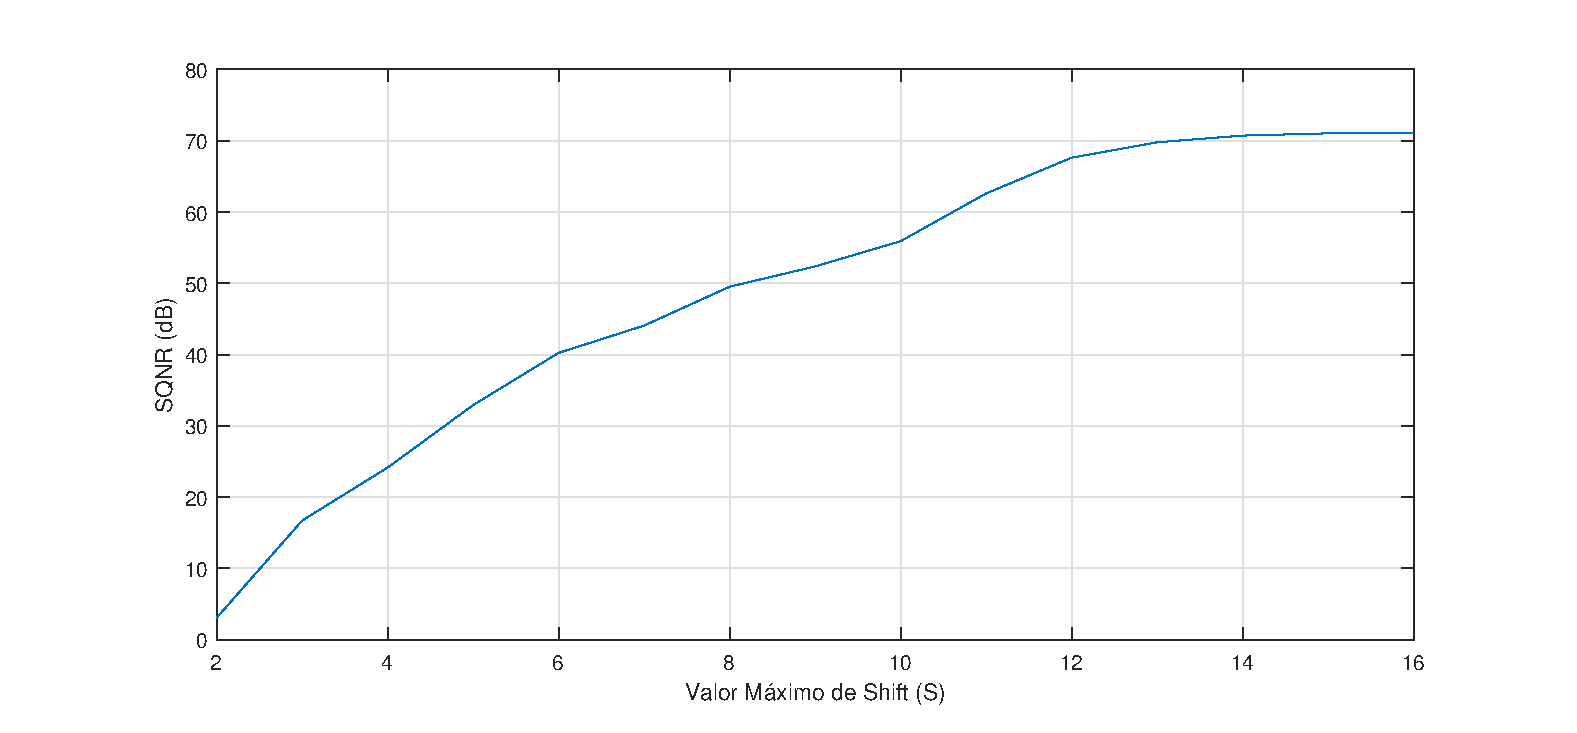
\includegraphics[width=0.9\linewidth]{Images/ImplementandoCordic/DeterminacaoS.eps}
	\caption{Rela��o entre $S$ e o SQNR M�dio para MSR Cordic Modo Normal}
	\vspace{-3.5mm}
	\caption*{Fonte: Autoria Pr�pria}
	\label{fig:DeterminacaoS}
\end{figure}    
\vspace{5mm}

Os conjuntos par�metros $s_i$ e $s_j$ para cada itera��o do algoritmo  ser�o armazenados em uma ROM de controle de cada Unidade Cordic. O n�mero de \textit{bits} necess�rios para armazenar estes par�metros � dado por $log(S)$. Como visto na Figura (\ref{fig:DeterminacaoS}) escolher $S=8$ promove um desempenho SQNR de $50dB$, e se faz necess�rio armazenar apenas $3$ \textit{bits} para cada elemento $s_i$ ou $s_j$. Por�m ao utilizar $4$ \textit{bits} para os mesmo fins � poss�vel fazer $S=16$, e alcan�ar um desempenho m�dio de $70dB$. Logo toma-se $S=16$ afim de alcan�ar o m�ximo desempenho poss�vel.

Com citado na Se��o (\ref{section:AnaliseDoErro}) os par�metros $I$ e $J$ podem ser constantes independente da opera��o de rota��o (Modo Normal), ou este podem variar a cada itera��o (Modo Generalizado). Com base no mesmo algoritmo implementado em $Matlab^\circledR$ apresentado anteriormente, foi inclu�do no vetor de �ngulos elementares $r$ as combina��es de par�metros poss�veis quanto tomado $N_{spt}=4$, para $(I=0,J=3)$,$(I=1,J=2)$, $(I=2,J=1)$ e $(I=3,J=0)$. E ent�o foram gerados os � conjuntos �timos de par�metros Cordic. 

O Modo Generalizado, para a simula��o proposta, apresentou um valor de SQNR de 92.9786 dB. O Modo Normal para o mesmo m�todo de simula��o apresentou um valor de 83.9786 dB. 

Segundo \cite{Chih}, para armazenar os par�metros $\{\mu_{i}, \mu_{j}\} \in \{-1,0, 1\}$, $\{s_i,s_j\} \in \{0,1,..,6\}$ de uma �nica intera��o do Algoritmo MSR Cordic, s�o necess�rios $(log(S)+2)N_{SPT}$ \textit{bits} para o modo Normalizado e $(log(S)+3)N_{SPT}$ para o Modo Generalizado. Ou seja o impacto do inser��o dos \textit{switches}, necess�rios no caso do Modo Generalizado, em termos de implementa��o � apenas a inclus�o de mais um \text{bit} no conjunto de dados de cada intera��o. Justificando portanto a escolha da implementa��o do MSR Cordic no Modo Generalizado.

Assim os dados referente aos par�metros escolhidos com base no Algoritmo (\ref{code:PCTBSAlterado}), para o MSR Cordic Modo Generalizado, com $N_{SPT}=3$ e $S=16$, s�o armazenados na forma bin�rio em uma componente ROM em VHDL. Esta ROM � presente e individual a cada unidade Cordic. 

\section{Arquitetura Cordic Implementada}
Ap�s a defini��o dos par�metros CORDIC, � ent�o realizada a implementa��o da arquitetura em FPGA, atrav�s da linguagem VHDL. Segundo \citeonline{Chih}, as opera��es de multiplica��o dos termos SPT em (\ref{eq:MSR}) podem ser realizadas utilizando operadores l�gicos de deslocamento de \textit{bit}, ou  \textit{shifters}. Como observado em (\ref{eq:MSR}), as duas partes $x$ e $y$ do sinal de entrada precisam ser deslocados para direita de forma diferenciada, com base nos par�metros $I$ e $J$, gerando assim cada parte $N_{SPT}$ sinais deslocados. 

As opera��es de deslocamento de $x$ e $y$ podem ser realizadas utilizando apenas dois \textit{Barrel shifters}, ambos com uma entrada e tr�s sa�das. O \textit{Barrel shifter} � um componentes l�gico capaz de deslocar um palavras bin�ria por um n�mero especifico de \textit{bits} utilizando apenas l�gica combinacional, o que possibilita efetuar a opera��o de deslocamento em apenas um ciclo de \textit{clock}. A �nica desvantagem deste componente � o n�mero elevado de multiplexadores necess�rios para sua implementa��o: $n log_2 n$, onde $n$ � o tamanho da palavra bin�ria. Por�m, como neste projeto $n=16$ \textit{bits}, admitiu-se o custo de inclus�o de 64 multiplexadores em prol de se obter o melhor desempenho na opera��o base do algoritmo CORDIC. 

Para a implementa��o em VHDL fora utilizado o diagrama de intera��o sugerido por \citeonline{Chih}, o qual segue na Figura (\ref{fig:ArquiteturaCordicGeneralizado}).

\vspace{5mm}
\begin{figure}[H]
	\centering
	\captionsetup{width=0.8\textwidth, font=footnotesize, textfont=bf}	
	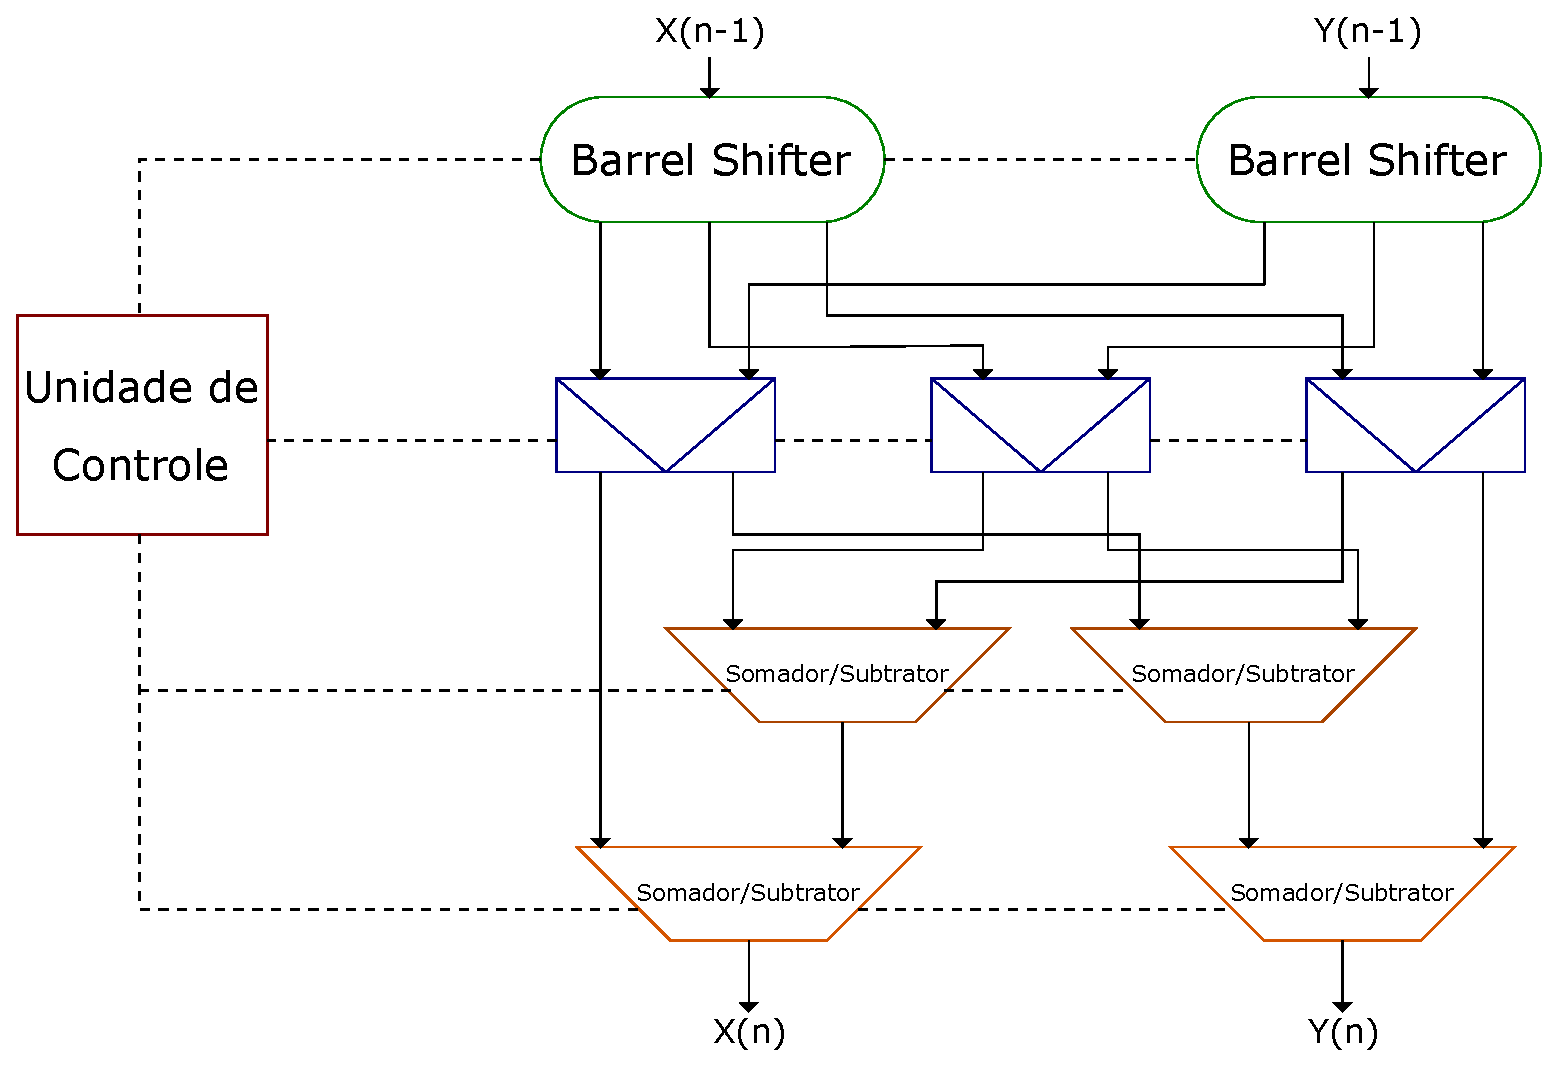
\includegraphics[width=0.8\linewidth]{Images/MateriaisMetodos/ArquiteturaCordicGeneralizado.eps}
	\caption{Arquitetura da Itera��o MSR Cordic Modo Normal $N_{spt}=3$}
	\vspace{-3.5mm}
	\caption*{Fonte: Adaptado \cite{Chih}}
	\label{fig:ArquiteturaCordicGeneralizado}
\end{figure}    
\vspace{5mm}

\vspace{5mm}
\begin{figure}[H]
	\centering
	\captionsetup{width=0.3\textwidth, font=footnotesize, textfont=bf}	
	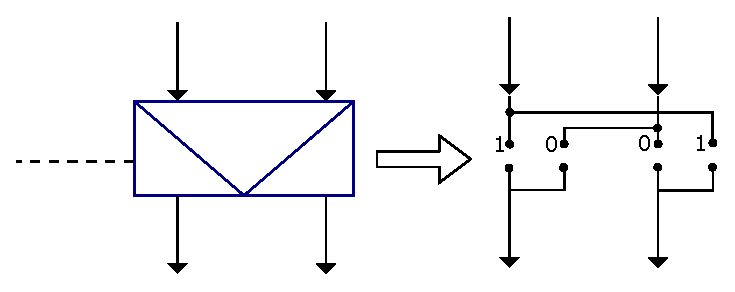
\includegraphics[width=0.3\linewidth]{Images/MateriaisMetodos/Sswitch.eps}
	\caption{Arquitetura Switch 2x2}
	\vspace{-3.5mm}
	\caption*{Fonte: Adaptado \cite{Chih}}
	\label{fig:Sswitch}
\end{figure}    
\vspace{5mm}

Como pode ser visto na Figura (\ref{fig:ArquiteturaCordicGeneralizado}), a implementa��o da intera��o CORDIC � feita basicamente de um conjunto de 4 somadores e 2 \textit{Barrel Shifters}. A implementa��o do Algoritmo CORDIC pode ser feita na forma sequencial ou na forma \textit{pipeline}. Na forma sequencial, a Unidade de Controle da Figura (\ref{fig:ArquiteturaCordicGeneralizado}), por meio de um conjunto de \textit{flip-flops}, armazenam o valor final da intera��o e retro alimentam a entrada do circuito, durante os $N$ ciclos de intera��o CORDIC. A cada intera��o a Unidade de Controle muda os par�metros de acordo com os dados presentes na ROM. Na forma de \textit{piperline} v�rias unidades CORDIC, como as vista Figura (\ref{fig:ArquiteturaCordicGeneralizado}), s�o encadeadas sequencialmente de modo que cada unidade seja respons�vel por uma intera��o separadamente, o que possibilita  a opera��o ser realizada em apenas um ciclo de \text{clock}.

Na forma sequencial a implementa��o do Algoritmo ocupa menos recursos da FPGA, j� que s�o necess�rios apenas um hardware de intera��o, e \textit{flip-flops} de controle. Apesar disso, o n�mero de ciclos de \textit{clock} necess�rios para concluir a opera��o � ditada pelas opera��es sequenciais do Unidade de Controle, que nunca ser� inferior a $N$ ciclos. Na forma \textit{pipeline}, o n�mero de ciclos de \textit{clock} necess�rios para finalizar a opera��o de rota��o  � dependente apenas da velocidade de propaga��o dos sinais, atrav�s do \textit{hardware} encadeado das itera��o. No entanto, como neste modo existem $N$ \textit{hardwares} de intera��o encadeados, o consumo de recursos da FPGA � bem maior. Por quest�o de limita��o de recursos da FPGA utilizada, se optou pela implementa��o na forma sequencial. 



 

